\documentclass[tikz,border=3.14mm]{standalone}

\begin{document}
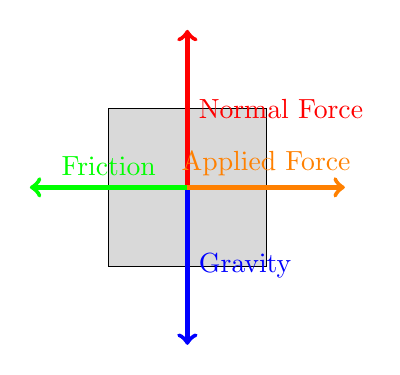
\begin{tikzpicture}
    % Draw the box
    \draw[fill=gray!30] (-1,-1) rectangle (1,1);

    % Draw the arrows representing forces
    \draw[->, ultra thick, blue] (0,0)--(0,-2) node[midway, right] {Gravity}; % down
    \draw[->, ultra thick, red] (0,0)--(0,2) node[midway, right] {Normal Force}; % up
    \draw[->, ultra thick, green] (0,0)--(-2,0) node[midway, above] {Friction}; % left
    \draw[->, ultra thick, orange] (0,0)--(2,0) node[midway, above] {Applied Force}; % right
\end{tikzpicture}
\end{document}